\documentclass[11pt,a4paper]{article}
\usepackage[a4paper,top=4cm,bottom=2.7cm,left=2.5cm,right=2.5cm]{geometry}
\usepackage{fontspec}
\setmainfont{Times New Roman}
\usepackage{microtype,graphicx,booktabs,tabularx,array,amsmath,amssymb}
\usepackage{caption,subcaption,xcolor,hyperref,natbib}
\hypersetup{colorlinks=true,allcolors=blue!55!black}
\captionsetup{font=small,labelfont=bf}
\setlength{\parindent}{2em}
\setlength{\parskip}{0pt}
\newcommand{\method}{Graph-Guided Nonlinear Evidence Navigation}
\IfFileExists{generated/results_macros.tex}{\newcommand{\TotalQuestions}{234}
\newcommand{\BestGraphMethod}{G5}
\newcommand{\BestGraphAcc}{53.85\%}
\newcommand{\BestGraphHardAcc}{42.86\%}
\newcommand{\TailAcc}{46.15\%}
\newcommand{\CompressAcc}{51.28\%}
\newcommand{\RAGAcc}{51.71\%}
\newcommand{\QZeroAcc}{40.17\%}
}{
  \newcommand{\TotalQuestions}{234}\newcommand{\BestGraphAcc}{pending}
  \newcommand{\BestGraphMethod}{G?}\newcommand{\TailAcc}{pending}
  \newcommand{\CompressAcc}{pending}\newcommand{\RAGAcc}{pending}
  \newcommand{\QZeroAcc}{pending}\newcommand{\BestGraphHardAcc}{pending}
}

\title{Beyond Linear Context: Graph-Guided Evidence Navigation for Long-Novel Reasoning with a Local 9B Language Model}
\author{Anonymous for review}
\date{}

\begin{document}
\maketitle

\begin{abstract}
Long-context question answering over novels requires a reader to connect characters, events, and evidence separated by tens of thousands of tokens. We study whether a frozen knowledge graph can convert this linear history into a navigable evidence structure for one fixed, local 9B language model. We reuse rather than rebuild 30 DetectiveQA novel graphs and evaluate five pre-specified graph routes against a tail window, ordinary whole-book compression, vector retrieval-augmented generation (RAG), and a question-only control. Gold paragraphs are withheld from retrieval and used only for post-hoc evaluation. We report question-level accuracy, a Q0-hard subset that excludes questions answerable without the novel, novel-macro accuracy, novel-clustered bootstrap intervals, paired McNemar tests, and graph-evidence concentration. Because the first 20 and final 10 graphs were produced by different frozen pipelines, their results are reported separately and the pooled result is explicitly descriptive. The best graph route obtains \BestGraphAcc\ accuracy on \TotalQuestions\ questions, compared with \TailAcc\ for the tail window, \CompressAcc\ for compression, and \RAGAcc\ for ordinary RAG. These experiments provide evidence about when nonlinear graph navigation helps a small-context reader, while avoiding causal claims from observational graph-layout statistics.
\end{abstract}

\noindent\textbf{Keywords:} long-context reasoning; knowledge graphs; retrieval-augmented generation; small language models; narrative question answering

\section{Introduction}
Increasing a model's nominal context window does not guarantee reliable use of information throughout that window. Relevant evidence placed in the middle can be used less effectively than evidence near the beginning or end \citep{liu2024lost,hsieh2024found}. This problem is acute in detective fiction: clues are dispersed, aliases and character relations evolve, and an answer may depend on several distant passages. DetectiveQA was designed around this setting and contains novel-length contexts with multi-evidence reasoning questions \citep{xu2024detectiveqa}.

We test a structural alternative to feeding a longer linear string. A novel graph makes characters, events, entities, and typed relations directly traversable. Question-conditioned retrieval can therefore jump across distant evidence without requiring the answering model to scan the entire narrative history. This is related to graph-based long-text agents \citep{li2024graphreader}, graph diffusion retrieval \citep{gutierrez2024hipporag}, hierarchical summarization \citep{sarthi2024raptor}, and GraphRAG \citep{edge2024graphrag}, but our target is deliberately narrower: a single local 9B model, no external API, no graph reconstruction during evaluation, and multiple-choice reasoning over full novels.

Our contributions are: (1) a hash-frozen 30-novel evaluation that holds the answering model and decoding protocol fixed; (2) a comparison of five graph routes with three non-graph baselines and a question-only contamination control; (3) an evidence-audit that separates retrieval recall from answer accuracy; and (4) a topological analysis of whether gold-overlap evidence is enriched in graph 2-cores, accompanied by a layout-sensitivity analysis and a preselected force-directed example.

\section{Related Work}
\subsection{Long-context utilization}
Lost-in-the-middle evaluations show that long-context performance depends strongly on evidence position \citep{liu2024lost}. Attention-bias calibration and position-agnostic training can improve utilization, but require model-level intervention or task-specific training \citep{hsieh2024found}. Our study instead changes the external evidence organization while leaving the local model fixed.

\subsection{Retrieval, compression, and graph navigation}
Standard RAG retrieves a small set of text passages before generation \citep{lewis2020rag}; LongRAG explores larger retrieval units for long-context models \citep{zhao2024longrag}. RAPTOR recursively summarizes and clusters passages into a tree \citep{sarthi2024raptor}. HippoRAG uses a knowledge graph and personalized PageRank for multi-hop integration \citep{gutierrez2024hipporag}. GraphReader lets an LLM agent plan and explore graph nodes under a small context window \citep{li2024graphreader}. That result is an important proof of concept, but its closed-model planning setup differs from our fixed local-model evaluation. GraphRAG targets query-focused summarization and combines graph community summaries with local evidence \citep{edge2024graphrag}; its global summarization objective should not be assumed to transfer directly to narrative multiple-choice reasoning.

\section{Materials and Methods}
\subsection{Frozen corpus and graph provenance}
We freeze 30 existing novel graphs before evaluation. The first cohort contains 20 legacy graphs; the second contains 10 Pass2-v4 graphs and includes novel 104. Each manifest entry records novel identifier, absolute source path, graph-builder lineage, node and edge counts, file size, modification time, and SHA-256 hash. Incomplete replacement graphs for novels 26--28 are excluded. The graph files are treated as immutable inputs, and hashes are checked before and after every new baseline run.

The two graph cohorts are heterogeneous by construction. Consequently, old20 and new10 are the primary reporting strata. Pooled 30-novel estimates are descriptive summaries and are not presented as if all graphs were generated by one pipeline.

\subsection{Model and controlled inference}
All newly executed conditions use the same local \texttt{qwen3.5:9b} model through Ollama, with reasoning disabled, fixed prompts, deterministic decoding settings, and a common context budget. No external API is used. Every question remains in the denominator. Output records retain the selected option, parse status, evidence payload, estimated input tokens where exact legacy token accounting is unavailable, elapsed time for new calls, model identity, and a run signature.

\subsection{Methods and baselines}
The five graph conditions (G1--G5) never consult a baseline prediction, gold answer, or gold paragraph. G1--G3 expose deterministic option-order permutations over the same graph evidence, G4 is their deterministic graph-only majority, and G5 is a tighter source-expansion traversal whose archived records explicitly set \texttt{baseline\_access=false}. These are five experimental conditions rather than five independent graph-construction algorithms. Because G4/G5 were selected or developed while inspecting this corpus, all five are labelled exploratory rather than a pristine held-out test. Earlier tail-fallback composites are retained in the historical archive but excluded from the main graph-method table.

Baselines are: B1, the final 50,000-character tail window; B2, ordinary whole-novel hierarchical compression within the same answer-model budget; and B3, ordinary vector RAG over contiguous text chunks without graph links. Q0 supplies only the question and options. Q0-hard removes questions answered correctly by Q0 from the evaluation subset; it does not mask options or modify any method input.

\subsection{Gold evidence isolation}
Gold clue and final-answer paragraphs are loaded only after graph freezing and prediction. They are used to score evidence overlap, never to retrieve, rank, route, or calibrate an answer. A graph node is marked as gold-overlap when its stored evidence and an annotated paragraph share a normalized substring of at least eight characters. This mechanical rule and the complete node-level audit table permit independent review.

\subsection{Dense-region analysis}
The primary topological definition collapses the graph to an undirected simple graph and marks nodes in its 2-core. For each cohort, we compute the gold-node core rate, non-gold rate, enrichment ratio, Haldane-corrected odds ratio, and novel-clustered bootstrap interval. A secondary visual definition marks nodes with undirected degree at least two whose normalized force-layout distance to the center is at most 0.45. Five fixed layout seeds quantify sensitivity. The topological definition supports statistical claims; the force-layout definition is descriptive.

\subsection{Statistical analysis}
We report micro accuracy and equal-weight novel-macro accuracy. Uncertainty uses a 95\% question-level Wilson interval and a 5,000-resample novel-clustered bootstrap. Graph--baseline comparisons use paired exact McNemar tests on the same questions with Holm correction over the planned family. We also report graph wins and losses, Q0-hard accuracy, and preservation among Q0-correct questions. No failed item is removed.

\section{Results}
\subsection{Answer accuracy}
Table~\ref{tab:main} and Figure~\ref{fig:accuracy} summarize the frozen evaluation. The best pooled graph route is \BestGraphMethod\ at \BestGraphAcc, while B1/B2/B3 obtain \TailAcc, \CompressAcc, and \RAGAcc, respectively; Q0 obtains \QZeroAcc. On Q0-hard questions, the best graph route obtains \BestGraphHardAcc. Statistical interpretation is based on paired wins/losses and corrected tests rather than point estimates alone.

\begin{table}[ht]
\centering
\caption{Accuracy on the frozen 30-novel evaluation. Pooled values are descriptive because graph construction differs across cohorts. Exact counts, macro averages, intervals, and Q0-hard values are generated from the archived per-question table.}
\label{tab:main}
\IfFileExists{generated/main_results_table.tex}{\begin{tabular}{lrrrr}
\toprule
Method & Correct & All & Novel macro & Q0-hard \\
\midrule
Graph order 1 & 118/234 & 50.43\% & 51.03\% & 37.14\% \\
Graph order 2 & 112/234 & 47.86\% & 48.02\% & 37.14\% \\
Graph order 3 & 118/234 & 50.43\% & 50.71\% & 39.29\% \\
Graph-only majority & 122/234 & 52.14\% & 52.81\% & 37.86\% \\
Tight graph expansion & 126/234 & 53.85\% & 53.34\% & 42.86\% \\
Tail window & 108/234 & 46.15\% & 45.27\% & 33.57\% \\
Whole-book compression & 120/234 & 51.28\% & 50.40\% & 37.14\% \\
Vector RAG & 121/234 & 51.71\% & 52.26\% & 36.43\% \\
Question only & 94/234 & 40.17\% & 40.66\% & -- \\
\bottomrule
\end{tabular}
}{\begin{tabular}{lcc}\toprule Method & All & Q0-hard\\\midrule Pending final aggregation & -- & --\\\bottomrule\end{tabular}}
\end{table}

\begin{figure}[ht]
\centering
\IfFileExists{generated/dqa30_accuracy.pdf}{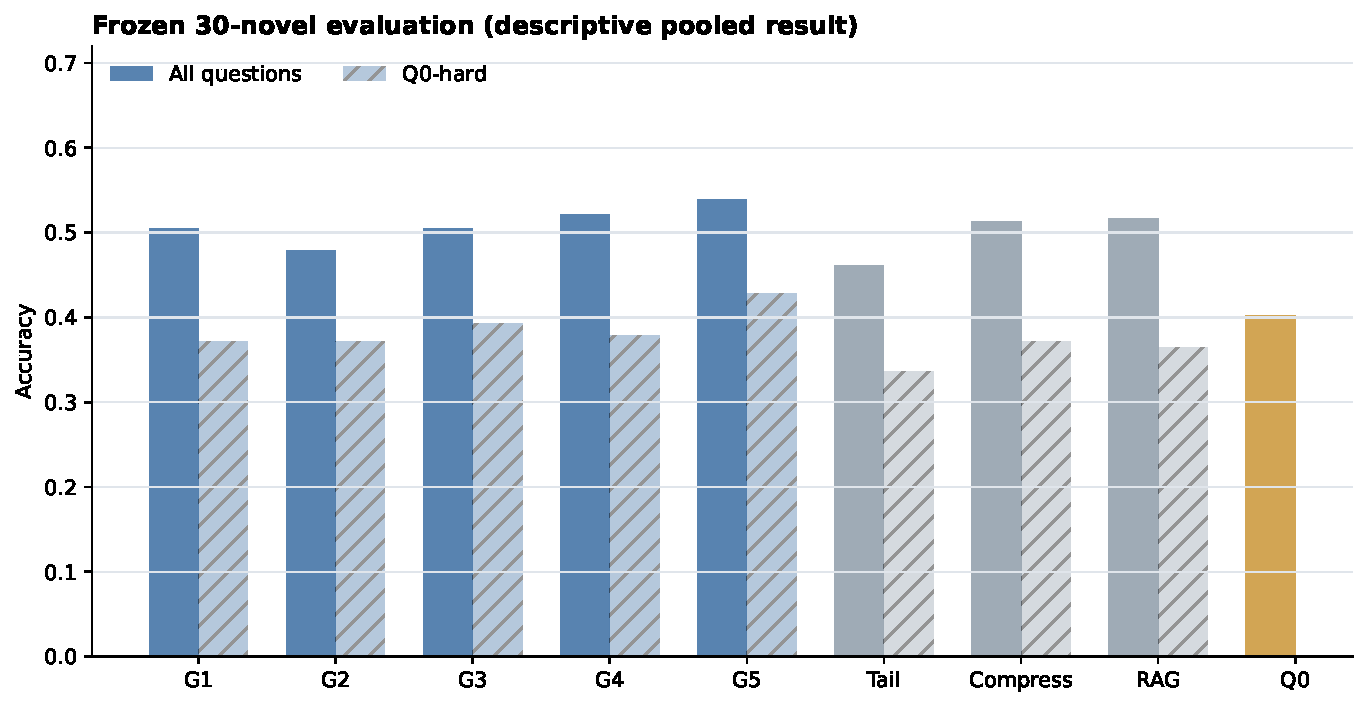
\includegraphics[width=0.98\linewidth]{generated/dqa30_accuracy.pdf}}{\fbox{Final accuracy figure pending}}
\caption{All-question and Q0-hard accuracy for five graph routes, three baselines, and Q0.}
\label{fig:accuracy}
\end{figure}

\subsection{Evidence concentration and graph quality}
Across the 20 legacy graphs, 66/123 gold-overlap nodes (53.66\%) and 1,835/10,095 other nodes (18.18\%) enter the 2-core, an enrichment of 2.95. Across the Pass2-v4 10, the corresponding values are 362/672 (53.87\%) and 1,524/4,557 (33.44\%), an enrichment of 1.61. The descriptive pooled enrichment is 2.35. Gold paragraph mapping recall differs sharply by cohort (16.32\% old20 versus 73.23\% new10), so this structural result cannot be interpreted without the build-version stratum.

\begin{figure}[ht]
\centering
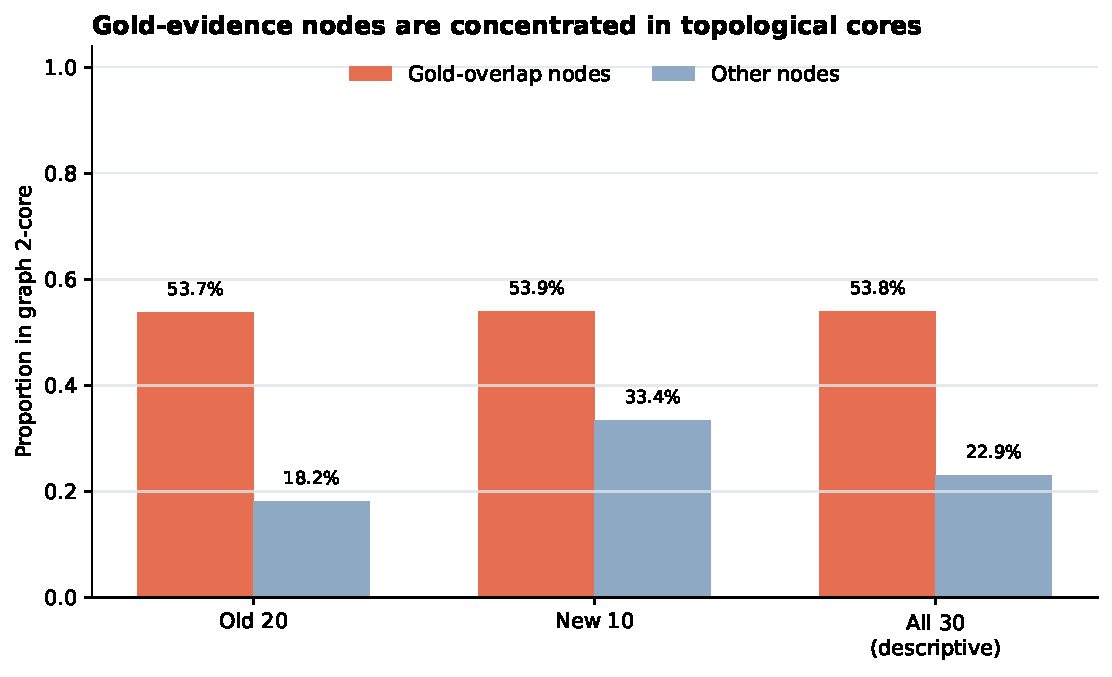
\includegraphics[width=0.76\linewidth]{generated/gold_dense_core_enrichment.pdf}
\caption{Gold-overlap nodes are enriched in graph 2-cores. This is an association between annotation overlap and topology, not a causal effect on model attention or accuracy.}
\label{fig:core}
\end{figure}

Novel 103 was selected before inspecting final answer performance to preserve continuity with an earlier research presentation. Figure~\ref{fig:force} displays its largest connected component for readability; density statistics use the complete graph.

\begin{figure}[ht]
\centering
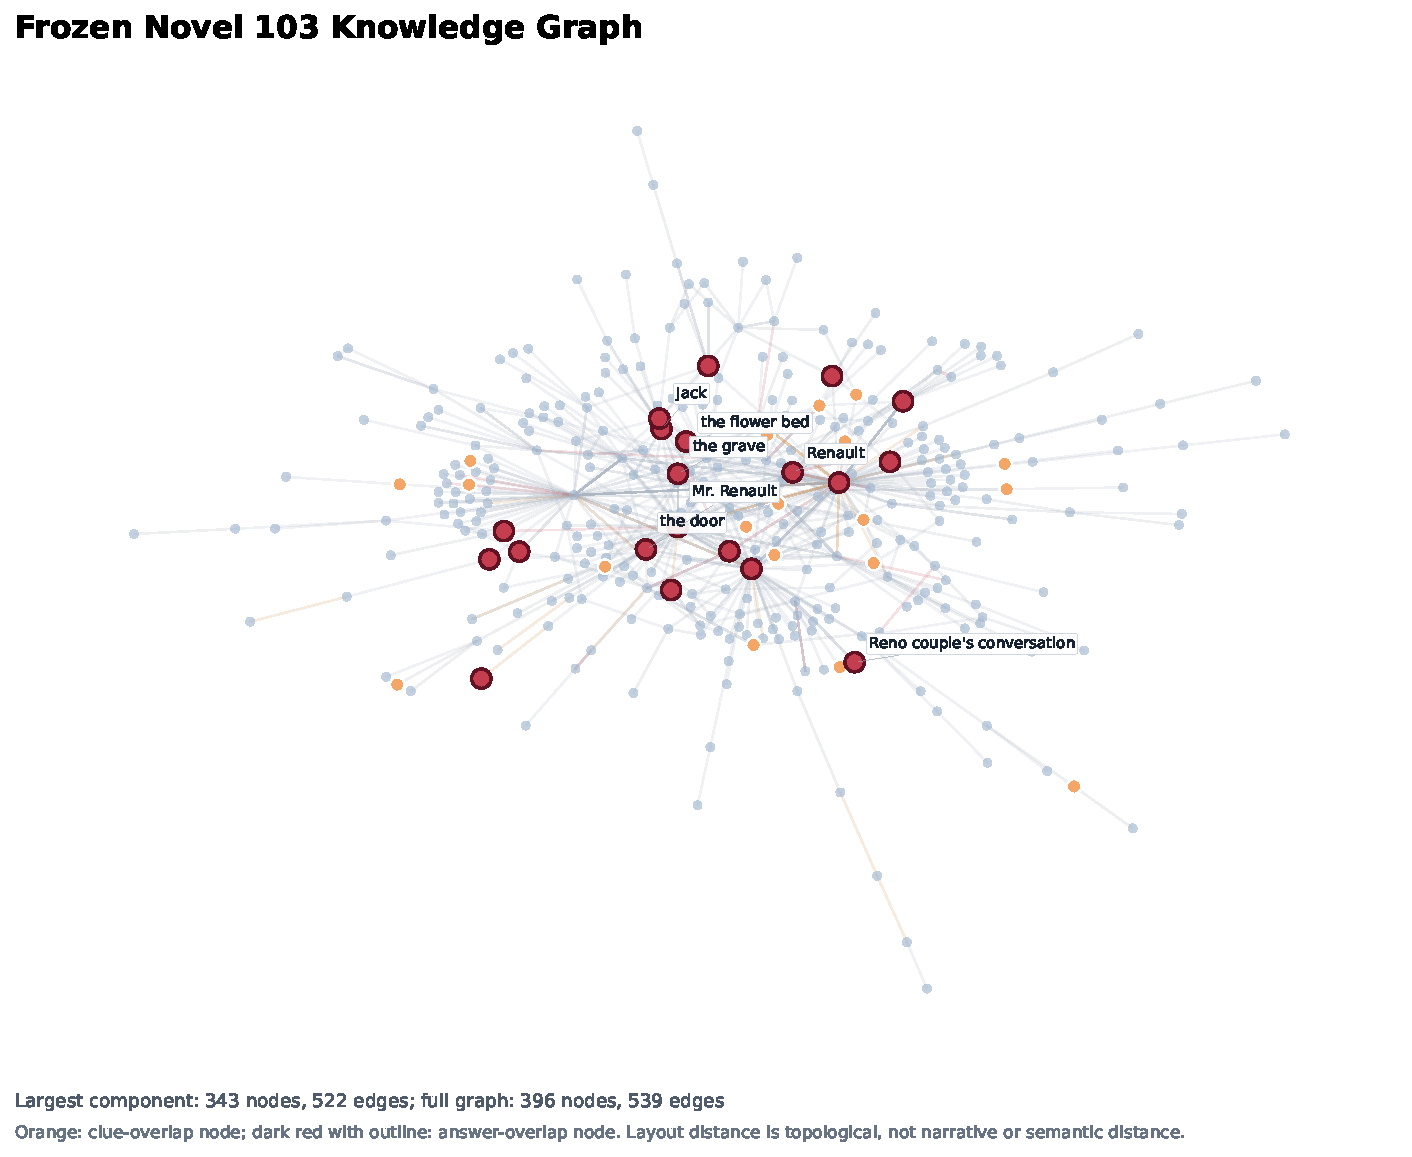
\includegraphics[width=0.98\linewidth]{generated/force_graph_novel103_paper.pdf}
\caption{Force-directed view of the frozen novel 103 graph. Orange nodes overlap clue paragraphs; dark red outlined nodes overlap final-answer paragraphs. Spatial distance is produced by topology and does not represent narrative time or semantic distance.}
\label{fig:force}
\end{figure}

\begin{figure}[ht]
\centering
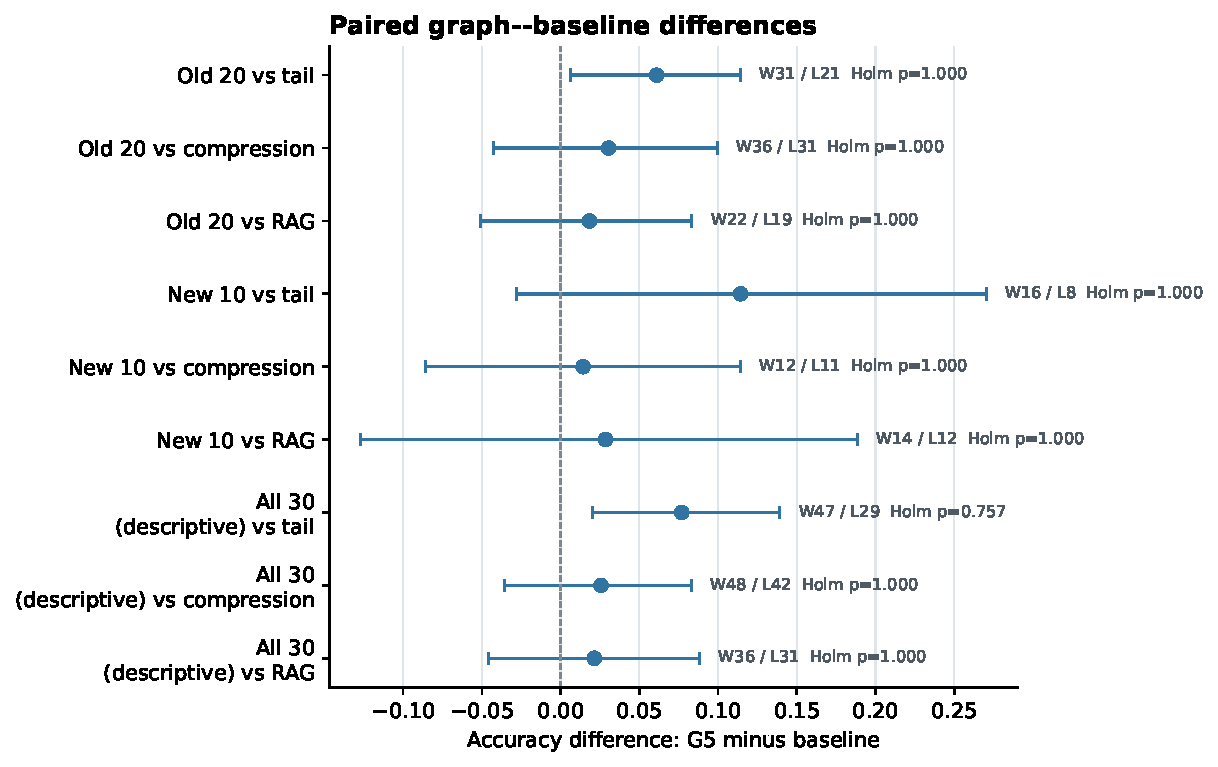
\includegraphics[width=0.92\linewidth]{generated/dqa30_pairwise.pdf}
\caption{Paired accuracy differences for the best pooled graph condition against each baseline, with novel-clustered bootstrap intervals and question-level wins/losses. Holm-adjusted values cover the 15 planned graph--baseline comparisons.}
\label{fig:paired}
\end{figure}

\begin{figure}[ht]
\centering
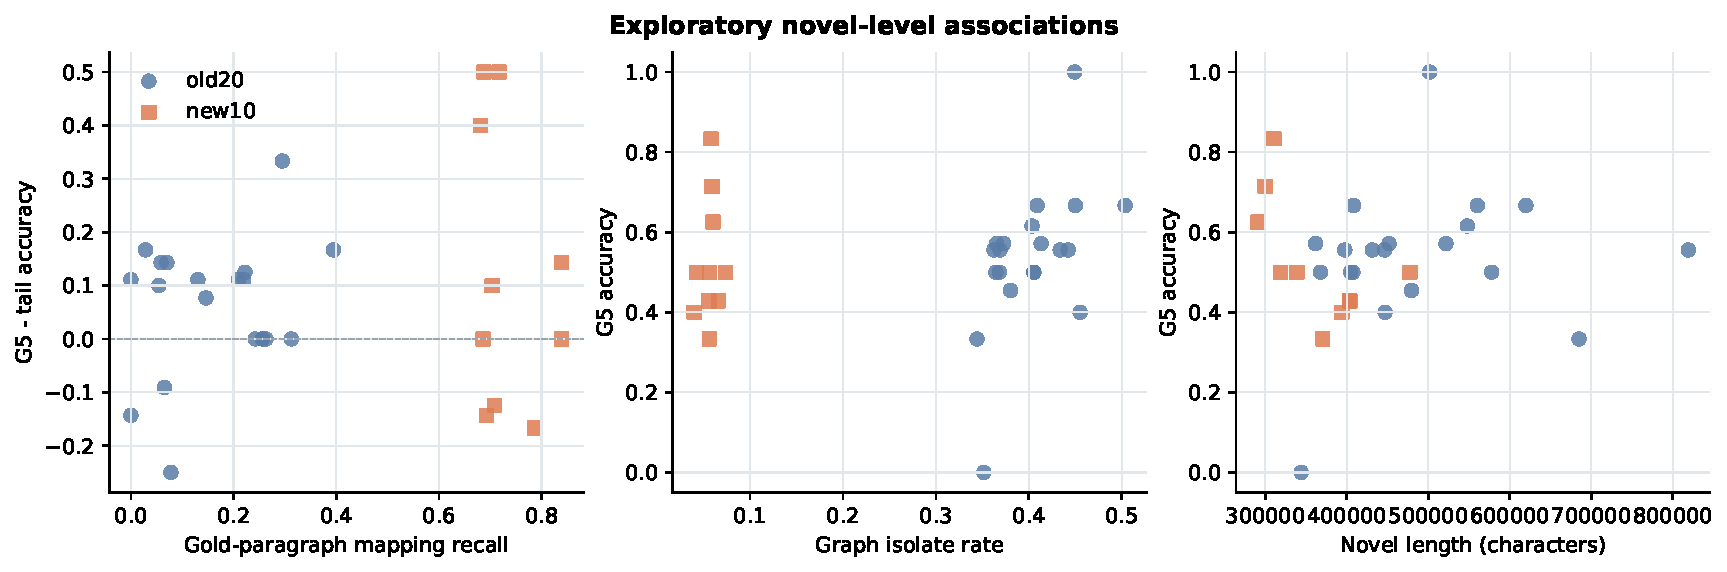
\includegraphics[width=0.98\linewidth]{generated/dqa30_relationships.pdf}
\caption{Exploratory novel-level relationships among gold-paragraph mapping recall, graph isolation, novel length, and G5 performance. Cohorts are shown separately; these associations are not causal tests.}
\label{fig:relationships}
\end{figure}

\section{Discussion}
The central hypothesis is structural: graph navigation can replace a portion of linear scanning with jumps between related evidence. A positive accuracy delta would support usefulness under the fixed local-model protocol, but it would not identify attention as the mechanism. Explicit transformer attention weights were not used as a primary endpoint because they are layer- and head-dependent and do not by themselves establish causal reliance. Evidence recall, context length, and answer correctness are therefore reported as distinct variables.

The strong cohort difference in paragraph mapping recall reveals a practical bottleneck. A graph may contain a visually dense core yet omit annotated evidence, and a retrieved gold paragraph may still fail to produce the correct answer. Improvements should therefore separate graph construction recall, question-conditioned traversal, context packing, and answer inference. Future confirmation should freeze one graph-building pipeline, pre-register one route, and evaluate on unseen novels.

\section{Limitations}
The sample contains 30 novels and 234 questions, with heterogeneous frozen graph pipelines. The graph routes were not all developed on a fully independent set. Some legacy runs preserve predictions and signatures but not exact tokenizer counts or per-call timings; those fields are explicitly marked unavailable rather than reconstructed as measurements. Gold-overlap uses a conservative lexical matching rule and can miss paraphrases. The force-directed view is seed-dependent, and its geometry is not evidence of semantic or temporal distance. Results apply to one local 9B answer model and should not be generalized to all small models without replication.

\section{Conclusion}
We provide a reproducible, graph-frozen evaluation of nonlinear evidence navigation for long-novel reasoning with one local 9B language model. The study design separates graph retrieval from gold evaluation, distinguishes question-only knowledge from text-derived gains, and reports graph-version heterogeneity rather than hiding it. The released manifests, hashes, per-question outputs, audit tables, scripts, and statistical tests make both positive and negative findings inspectable.

\bibliographystyle{plainnat}
\bibliography{references}
\end{document}
